\documentclass[../main.tex]{subfiles}

\begin{document}
    \section{List}
    List is a kind of data structure that can handle data whose size changes
    while program is running. For example, you want to write a program that can
    manage your shopping list. When you go shopping, you are adding and removing
    items to and from this list, and you are not very likely to know what items
    and how many of them you are going to buy. A list offers a solution to this
    kind of problem.

    You can imagine that a list is an array with changable size.

    A list can perform following operations:
    \begin{itemize}
        \item Add an item: \texttt{Add}
        \item Remove an item from list: \texttt{Remove}
        \item Find if an item is in list: \texttt{Contains}
        \item Get the index of an item that is in list: \texttt{Find}
        \item Insert an item at a specific location in list: \texttt{Insert}
    \end{itemize}

    Here is how a list could look like in the memory of a computer:
    
    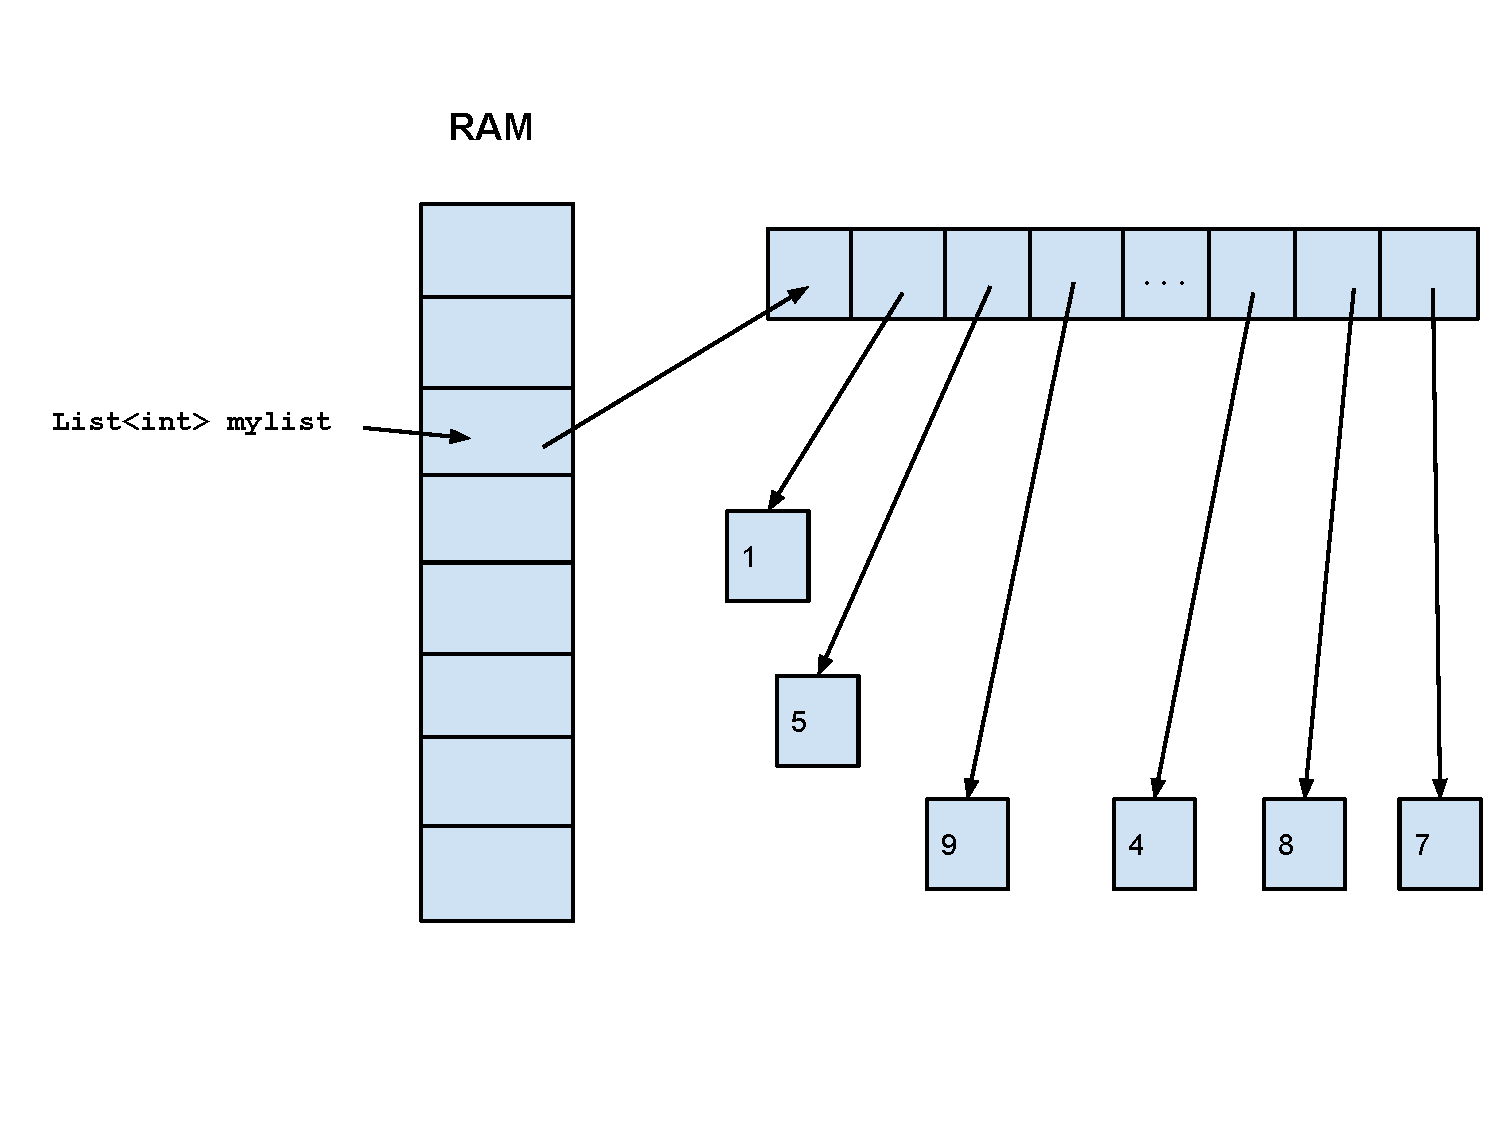
\includegraphics[scale = 0.5]{data/img/mmap-list.pdf}
\end{document}
